% This is a simple template for a LaTeX document using the "article" class.
% See "book", "report", "letter" for other types of document.

\documentclass[10pt]{article} % use larger type; default would be 10pt

\usepackage[utf8]{inputenc} % set input encoding (not needed with XeLaTeX)

%%% Examples of Article customizations
% These packages are optional, depending whether you want the features they provide.
% See the LaTeX Companion or other references for full information.

%%% PAGE DIMENSIONS
\usepackage{geometry} % to change the page dimensions
\geometry{a4paper} % or letterpaper (US) or a5paper or....
\usepackage{setspace}
\usepackage{parskip}
\parskip = 0.3 \baselineskip %\advance\parskip by 0pt plus 2pt% to change between paragraphs space
% \geometry{margin=2in} % for example, change the margins to 2 inches all round
% \geometry{landscape} % set up the page for landscape
%   read geometry.pdf for detailed page layout information

% \usepackage{gravarphicx} % support the \includegravarphics command and options
% \usepackage[parfill]{parskip} % Activate to begin paragraphs with an empty line rather than an indent

%%% PACKAGES
\usepackage{{booktabs}} % for much better looking tables
\usepackage{array} % for better arrays (eg matrices) in maths
\usepackage{paralist} % very flexible & customisable lists (eg. enumerate/itemize, etc.)
\usepackage{verbatim} % adds environment for commenting out blocks of text & for better verbatim
\usepackage{subfig} % make it possible to include more than one captioned figure/table in a single float
% These packages are all incorporated in the memoir class to one degree or another...
\usepackage[fleqn]{amsmath}
\usepackage{amssymb}
\usepackage{enumitem}
\usepackage{amsthm}
\usepackage{graphicx}
\usepackage{filecontents}
\usepackage{natbib}
\usepackage{blindtext}
\usepackage{titlesec}
\usepackage[table,xcdraw]{xcolor}


%%% HEADERS & FOOTERS
\usepackage{fancyhdr} % This should be set AFTER setting up the page geometry
\pagestyle{plain} % options: empty , plain , fancy
\renewcommand{\headrulewidth}{0pt} % customise the layout...
\lhead{}\chead{}\rhead{}
\lfoot{}\cfoot{\thepage}\rfoot{}

%%% SECTION TITLE APPEARANCE
\usepackage{sectsty}
\allsectionsfont{\rmfamily\bfseries\upshape} % (See the fntguide.pdf for font help)
% (This matches ConTeXt defaults)

%%% ToC (table of contents) APPEARANCE
\usepackage[nottoc,notlof,notlot]{tocbibind} % Put the bibliography in the ToC
\usepackage[titles,subfigure]{tocloft} % Alter the style of the Table of Contents
\renewcommand{\cftsecfont}{\rmfamily\mdseries\upshape}
\renewcommand{\cftsecpagefont}{\rmfamily\mdseries\upshape} % No bold!

\usepackage[colorlinks,citecolor=black,urlcolor=black,bookmarks=false,hypertexnames=true]{hyperref} 

%%% END Article customizations



%%% The "real" document content comes below...

\title{MECON6102 Problem Set 1}
\author{Xing Mingjie}
\date{\today} % Activate to display a given date or no date (if empty),
         % otherwise the current date is printed 

\begin{document}
\maketitle

% \tableofcontents

\begin{abstract}
    This report studies the relationship between monthly stock returns and a set of factors and construct an investment strategy based on various factor models. The report first uses a naive factor regression to estimate the factor loadings of the stock returns. Then, the report uses the Fama-MacBeth regression to estimate the factor risk premia. Finally, the report uses the LASSO regression to select the factors. The report also constructs a mean-variance portfolio based on the factor risk premia.
\end{abstract}

\section{Data}
The stock monthly return data is obtained from the CRSP database. The sample creates an unbalanced panel of 573 stocks from 2000-01 to 2022-12. There are in total 82060 observations.

The factors combine Fama-French 5 factors model, q-Factor of \cite{HouXueZhang2014}, and liquidity factor of \cite{PastorStambaugh2003}. Readers are referred to the juoyter notebook for detailed description of the factors.

\subsection{Data preparation}
    To boost calculation, regressions in this exercise is performed on a rolling window with size of 60. So those stocks with less than 60 observations are dropped. The final panel consists of 78233 observations of 390 stocks.
\section{Naive Factor Regression}

\begin{figure}
    \centering
    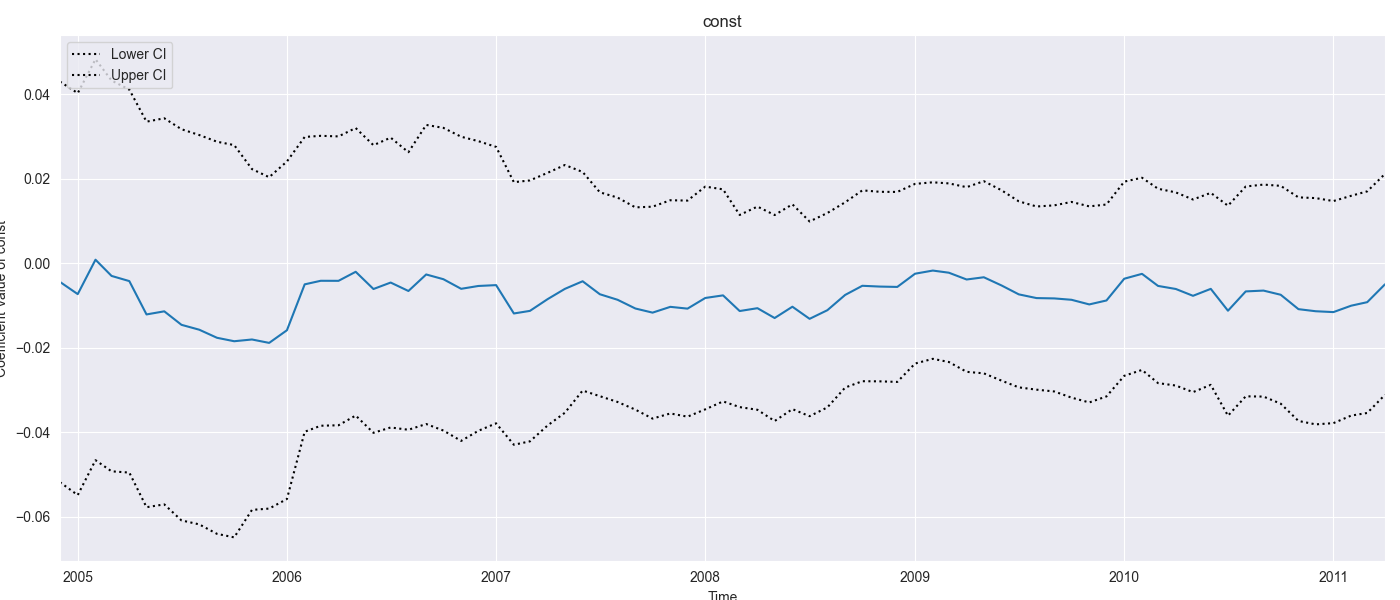
\includegraphics[width=0.8\textwidth]{"../fig/const_naive_coeff.png"}
    \caption{$\alpha$ time series of stock 10324}
    \label{fig:const_naive_coeff}
\end{figure}

In Figure \ref{fig:const_naive_coeff} we can see that the intercept term $\alpha$ is relatively stable over time, oscilliating around -0.01. This is consistent with the theory that the intercept term should be zero in the textbook CAPM model. The small negativity of the intercept could be due to the fact that the stock \texttt{10324} loses to the market in the sample period, and having a negative risk premium, especially in the early 2005.

\begin{figure}
    \centering
    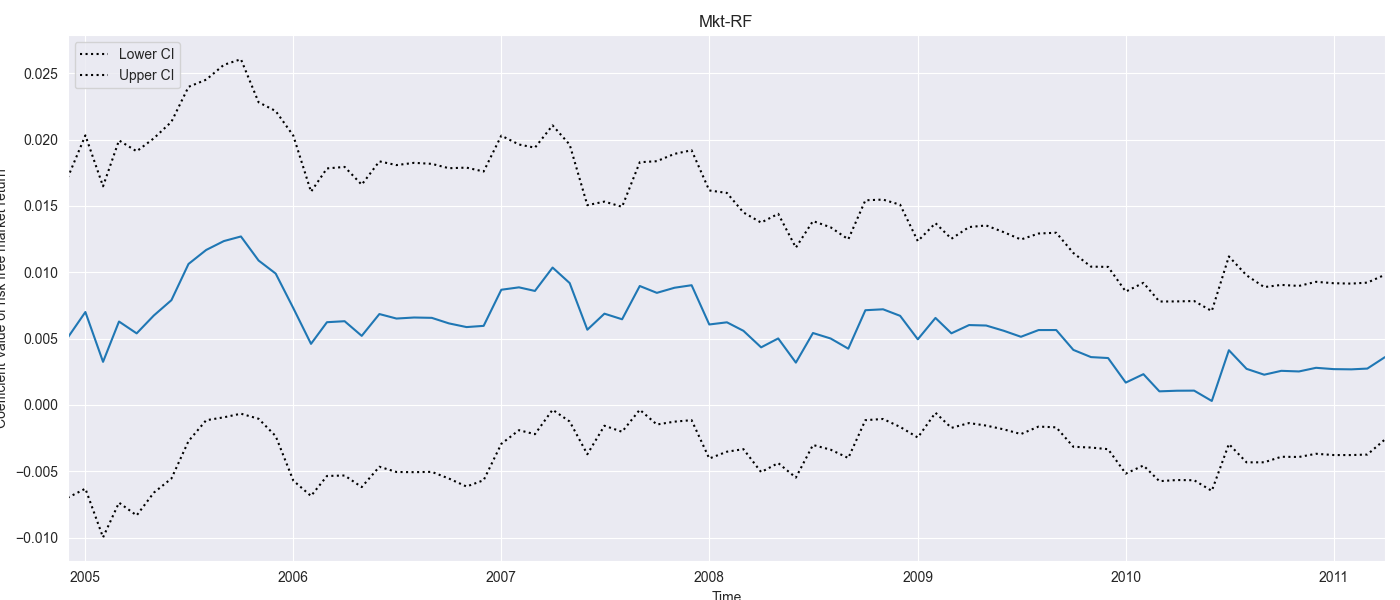
\includegraphics[width=0.8\textwidth]{"../fig/mktrf_naive_coeff.png"}
    \caption{$\beta_{Mkt-RF}$ time series of stock 10324}
    \label{fig:mktrf_naive_coeff}
\end{figure}
In Figure \ref{fig:mktrf_naive_coeff} we can see the risk exposure to market risk free return is arguably consistent acorss time, around 0.005, though there is a secular downward trend, especially since the surge in late 2005. This is consistent with the theory that the market risk premium should be positive and stable over time. The decreasing trend may be due to the fact that the stock \texttt{10324} is becoming less risky over time, or the market is becoming more risky over time.

\section{Fama-MacBeth Regression}
\begin{figure}
    \centering
    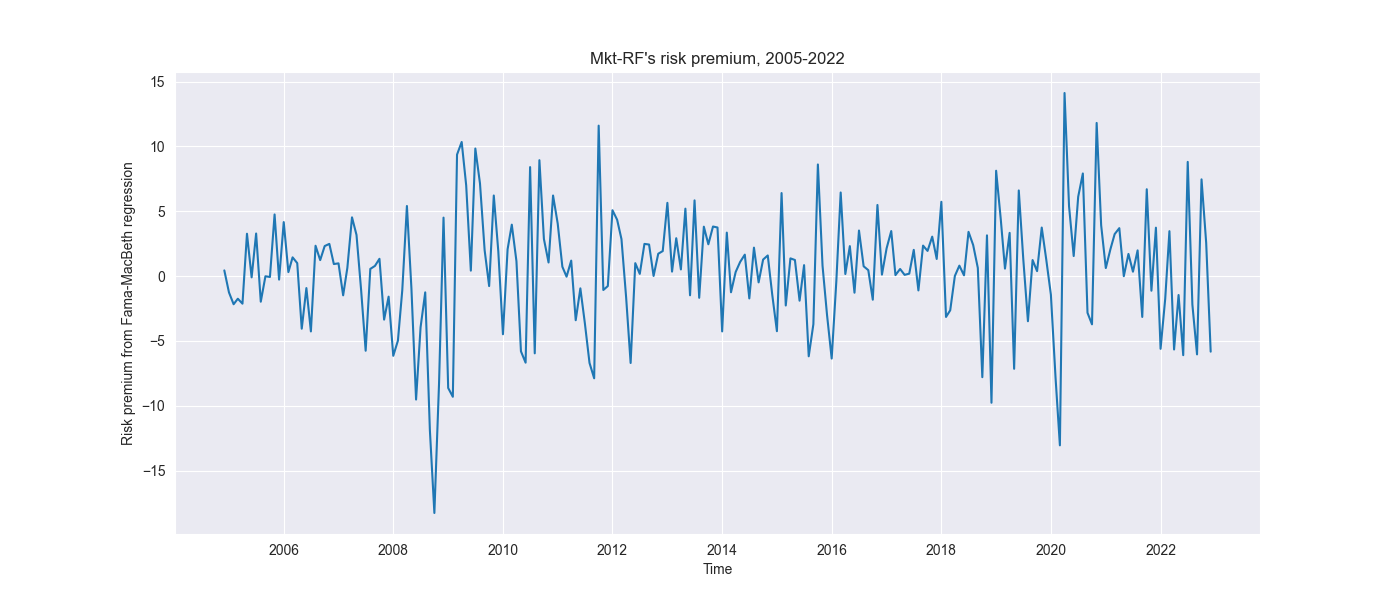
\includegraphics[width=1\textwidth]{"../fig/mktrf_fm_riskp.png"}
    \caption{$\gamma_{Mkt-RF}$ risk premium time series}
    \label{fig:mktrf_fm_riskp}
\end{figure}
In Figure \ref{fig:mktrf_fm_riskp} we can see the risk premium of the market risk free return is oscilliating around 0. The negative most value happens in late 2008, possibly due to the financial crisis. The stability of the risk premium is also consistent with the stability of the risk exposure to market risk free return in the naive factor regression.


\section{LASSO Regression}
Factors are lagged by one to six months to avoid look-ahead bias. First 5 rows of each window are dropped due to missing value in the lagged factors.

\begin{table}
\caption{Top 5 factors selected by LASSO each period}
\label{tab:top5factor}
\begin{tabular}{llllll}
\toprule
 & 1st & 2nd & 3rd & 4th & 5th \\
date &  &  &  &  &  \\
\midrule
200501 & Mkt-RF & HML & Mkt-RF-l5 & HML-l3 & Mkt-RF-l4 \\
200601 & Mkt-RF & Mkt-RF-l2 & HML & Mkt-RF-l5 & Mkt-RF-l4 \\
200701 & Mkt-RF & R_ME & SMB & Mkt-RF-l3 & Mkt-RF-l1 \\
200801 & Mkt-RF & Mkt-RF-l2 & SMB & Mkt-RF-l1 & HML \\
200901 & Mkt-RF & Mkt-RF-l3 & HML & Mkt-RF-l1 & Mkt-RF-l4 \\
201001 & Mkt-RF & Mkt-RF-l4 & Mkt-RF-l1 & Mkt-RF-l2 & Mkt-RF-l3 \\
201101 & Mkt-RF & Mkt-RF-l1 & Mkt-RF-l4 & Mkt-RF-l2 & HML \\
201201 & Mkt-RF & Mkt-RF-l2 & Mkt-RF-l4 & Mkt-RF-l1 & Mkt-RF-l3 \\
201301 & Mkt-RF & Mkt-RF-l4 & Mkt-RF-l2 & Mkt-RF-l1 & Mkt-RF-l3 \\
201401 & Mkt-RF & Mkt-RF-l6 & Mkt-RF-l5 & Mkt-RF-l4 & Mkt-RF-l2 \\
201501 & Mkt-RF & Mkt-RF-l1 & Mkt-RF-l6 & Mkt-RF-l2 & Mkt-RF-l3 \\
201601 & Mkt-RF & Mkt-RF-l3 & Mkt-RF-l6 & R_ME & Mkt-RF-l1 \\
201701 & Mkt-RF & HML & Mkt-RF-l3 & Mkt-RF-l5 & Mkt-RF-l1 \\
201801 & Mkt-RF & HML & SMB & Mkt-RF-l1 & R_ME \\
201901 & Mkt-RF & HML & Mkt-RF-l1 & Mkt-RF-l5 & Mkt-RF-l4 \\
202001 & Mkt-RF & HML & Mkt-RF-l1 & Mkt-RF-l3 & Mkt-RF-l4 \\
\bottomrule
\end{tabular}
\end{table}
}

LASSO exercise is done without cross validation. The step size is chosen at 0.001. Risk free market return is chosen as the most prevalent factor in the LASSO regression throughout the time, as can be seen in Table \ref{tab:top5factor}. This is in line with the L2-Boosting result. Other factors that are frequently chosen include \texttt{HML}, \texttt{SMB}, \texttt{R\_ME}, and 1 to 6 month lag of risk free market return. \texttt{SMB} is the size factor, \texttt{HML} is the value factor, and \texttt{R\_ME} is the momentum factor. These findings are also consistent with the Gradient Boosting result.

\section{Mean-Variance Portfolio}

\section{Conclusion}

\newpage
\footnotesize
\bibliographystyle{apalike}
\bibliography{ref}

\end{document}